Durante lo sviluppo del progetto ci siamo affidati al test driven development per avere la garanzia del comportamento atteso.

Il test driven development (TDD) � una tecnica di programmazione che prevede la scrittura di un test, ovvero di una porzione di codice che si occupa di verificare una funzionalit�, prima della stesura della funzionalit� stessa.

>per scrivere i test si utilizzano appositi \textit{framework} specifici per ogni linguaggio.

>I test posso essere soddifatti e sono definiti green o falliti e sono definiti red, questa nomenclatura deriva dalle usuali convenzioni degli ambienti di test che utilizzano questi colori per rappresentare il successo o meno di un test.

L'ideazione e la diffusione di questa tecnica di programmazione � stata curata da Kent Beck, che nel suo libro \textit{Test Driven Development: By Example} \cite{Beck:2002:TDD:579193} spiega come applicare il TDD a svariati contesti  legati allo sviluppo e dettaglia questa tecnica nelle sue tre fasi fondamentali definite abitualmente con il termine \textit{red-green-refactor}. Vediamo nel dettaglio cosa si intende con questo concetto.

\begin{description}
\item[Prima fase: red] Ogni nuova feature da implementare inizia con la stesura di un nuovo test, questo aiuta il programmatore a definire a priori le specifiche funzionali della porzione di sistema che dovr� implementare. La funzionalit� descritta dal test pu� mappare direttamente una \textit{user story} o pu� essere una porzione di essa. Non avendo implementato la funzionalit� il test sar� rosso (fallito). (verifica del test stesso?)
\item[Seconda fase: green] Questa fase del processo � quella nella quale si esegue lo sviluppo vero e proprio della funzionalit�, in modo da far diventare il test verde (soddisfatto). L'obbiettivo � esclusivamente soddisfare i requisiti, quindi tipicamente lo sviluppatore cerca di arrivare alla soluzione nel modo pi� semplice possibile, non curandosi dei dettagli stilistici del codice.
\item[Terza fase: refactor] L'ultimo passo da eseguire � la rifattorizzazione del codice, cio� la riorganizzazione delle funzionalit� realizzate al passo precedente al fine di ottenere una architettura ben congegnata e una struttura chiara. Una delle tecniche principali per realizzare questo compito � chiamata \textit{Don't Repeat Yourself} (DRY) e consiste nel cercare di rimuovere quanto pi� possibile codice duplicato mantenendo le stesse funzionalit�. L'utilizzo di questa tecnica favorisce il riuso e, tipicamente, veicola verso un buon design del software. In questa fase lo sviluppatore ha la massima libert� di sperimentazione, in quanto la correttezza del software rifattorizzato � garantita dai test scritti in precedenza. 
\end{description}

\begin{figure}[h]
\centering
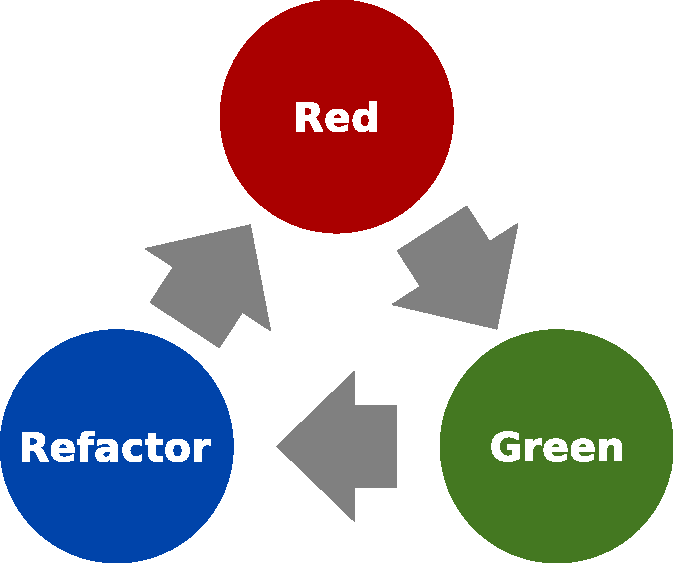
\includegraphics[width=0.7\linewidth]{./img/red-green-refactor}
\caption[Il flusso di lavoro del TDD]{Il flusso di lavoro del TDD}
\label{fig:red-green-refactor}
\end{figure}

Il processo � iterativo e ricomincia da capo

L'utilizzo del TDD fornisce allo sviluppatore svariati vantaggi, ad esempio:

- si riduce molto la necessit� di un debugger
- il programmatore acquisisce fiducia e non � pi� spaventato dal refactoring del codice, permette al programmatore di sperimentare soluzioni azzardate senza paura
- i test fungono da documentazione del codice e da traccia dello stato di avanzamento del progetto
- aiuta a modularizzare il codice e a realizzarlo in unit� indipendenti tra loro.
- favorisce il "concentrarsi sulle funzionalit�" e garantisce che ogni funzionalit� sia verificata con un test.




%TDD
%Il Test Driven Development, in sigla TDD (in italiano: Sviluppo guidato dalle verifiche) � un processo di sviluppo del software in cui lo sviluppo vero e proprio � preceduto (e guidato, driven) dalla stesura di test automatici.
%Sviluppato e diffuso da Kent Beck, fa parte delle 12 regole alla base dell'Extreme Programming (XP). Mentre XP � una metodologia agile, il TDD � una pratica agile.

%Il processo si articola sulla ripetizione di brevi cicli di sviluppo e collaudo (noti come "cicli TDD", TDD cycles) suddivisi in tre fasi successive, sintetizzate dal motto "Red-Green-Refactor".
%nella prima ("Red"), il programmatore scrive un test automatico (che necessariamente fallisce) per la funzionalit� da sviluppare.
%nella seconda ("Green"), il programmatore scrive la quantit� minima di codice necessaria per ottenere il superamento del test.
%nella terza, il programmatore ristruttura il codice (ovvero ne fa il refactoring).
%I colori "rosso" e "verde" si riferiscono alla rappresentazione grafica di fallimento e successo di un test automatico pi� diffusa negli IDE.
%Vantaggi
%Tali test permettono di individuare con precisione le specifiche del codice, e quindi il suo comportamento in base alle situazioni a cui sar� sottoposto. Ci� facilita la produzione di un codice funzionante in qualunque circostanza, pi� pulito e pi� affidabile.
%Scrivendo i test prima del codice, si utilizza il programma prima ancora che venga realizzato. Ci si assicura, inoltre, che il codice prodotto � testabile singolarmente. � dunque obbligatorio avere una visione precisa del modo in cui verr� utilizzato il programma prima ancora d'essere implementato. Cos� facendo si evitano errori concettuali durante la realizzazione dell'implementazione, senza che si siano definiti gli obiettivi. Inoltre, i test consentono agli sviluppatori di avere maggior confidenza durante il refactoring del codice, in quanto gi� sanno che i test funzioneranno quando richiesto; pertanto, possono permettersi di effettuare cambiamenti radicali di design, stando certi che alla fine otterranno un programma che si comporter� sempre alla stessa maniera (essendo i test sempre verificati).
%L'uso del Test Driven Development permette non solo di costruire il programma assieme ad una serie di test di regressione automatizzabili, ma anche di stimare in maniera pi� precisa lo stato d'avanzamento dello sviluppo di un progetto.

%------------------------------------------------------------------------------

%Test-driven development (TDD) is a software development process that relies on the repetition of a very short development cycle: first the developer writes an (initially failing) automated test case that defines a desired improvement or new function, then produces the minimum amount of code to pass that test, and finally refactors the new code to acceptable standards. Kent Beck, who is credited with having developed or 'rediscovered' the technique, stated in 2003 that TDD encourages simple designs and inspires confidence.[1]
%Test-driven development is related to the test-first programming concepts of extreme programming, begun in 1999,[2] but more recently has created more general interest in its own right.[3]
%Programmers also apply the concept to improving and debugging legacy code developed with older techniques.[4]

%The following sequence is based on the book Test-Driven Development by %Example.[1]
%Add a test[edit]
%In test-driven development, each new feature begins with writing a test. This test must inevitably fail because it is written before the feature has been implemented. (If it does not fail, then either the proposed "new" feature already exists or the test is defective.) To write a test, the developer must clearly understand the feature's specification and requirements. The developer can accomplish this through use cases and user stories to cover the requirements and exception conditions, and can write the test in whatever testing framework is appropriate to the software environment. This could also be a modification of an existing test. This is a differentiating feature of test-driven development versus writing unit tests after the code is written: it makes the developer focus on the requirements before writing the code, a subtle but important difference.
%Run all tests and see if the new one fails[edit]
%This validates that the test harness is working correctly and that the new test does not mistakenly pass without requiring any new code. This step also tests the test itself, in the negative: it rules out the possibility that the new test always passes, and therefore is worthless. The new test should also fail for the expected reason. This increases confidence (though does not guarantee) that it is testing the right thing, and passes only in intended cases.
%Write some code[edit]
%The next step is to write some code that causes the test to pass. The new code written at this stage is not perfect, and may, for example, pass the test in an inelegant way. That is acceptable because later steps improve and hone it.
%At this point, the only purpose of the written code is to pass the test; no further (and therefore untested) functionality should be predicted and 'allowed for' at any stage.
%Run tests[edit]
%If all test cases now pass, the programmer can be confident that the code meets all the tested requirements. This is a good point from which to begin the final step of the cycle.
%Refactor code[edit]
%Now the code should be cleaned up as necessary. Move code from where it was convenient for passing the test to where it logically belongs. Remove any duplication you can find. Make sure that variable and method names represent their current use. Clarify any constructs that might be misinterpreted. Use Kent Beck's four rules of simple design[5][6] to guide you, as well as anything else you know about writing clean code. By re-running the test cases, the developer can be confident that code refactoring is not damaging any existing functionality.
%The concept of removing duplication is an important aspect of any software design. In this case, however, it also applies to removing any duplication between the test code and the production code?for example magic numbers or strings repeated in both to make the test pass in step 3.
%Repeat[edit]
%Starting with another new test, the cycle is then repeated to push forward the functionality. The size of the steps should always be small, with as few as 1 to 10 edits between each test run. If new code does not rapidly satisfy a new test, or other tests fail unexpectedly, the programmer should undo or revert in preference to excessive debugging. Continuous integration helps by providing revertible checkpoints. When using external libraries it is important not to make increments that are so small as to be effectively merely testing the library itself,[3] unless there is some reason to believe that the library is buggy or is not sufficiently feature-complete to serve all the needs of the main program being written.

%Benefits[edit]

%A 2005 study found that using TDD meant writing more tests and, in turn, programmers who wrote more tests tended to be more productive.[11] Hypotheses relating to code quality and a more direct correlation between TDD and productivity were inconclusive.[12]
%Programmers using pure TDD on new ("greenfield") projects reported they only rarely felt the need to invoke a debugger. Used in conjunction with a version control system, when tests fail unexpectedly, reverting the code to the last version that passed all tests may often be more productive than debugging.[13]
%Test-driven development offers more than just simple validation of correctness, but can also drive the design of a program.[citation needed] By focusing on the test cases first, one must imagine how the functionality is used by clients (in the first case, the test cases). So, the programmer is concerned with the interface before the implementation. This benefit is complementary to Design by Contract as it approaches code through test cases rather than through mathematical assertions or preconceptions.
%Test-driven development offers the ability to take small steps when required. It allows a programmer to focus on the task at hand as the first goal is to make the test pass. Exceptional cases and error handling are not considered initially, and tests to create these extraneous circumstances are implemented separately. Test-driven development ensures in this way that all written code is covered by at least one test. This gives the programming team, and subsequent users, a greater level of confidence in the code.
%While it is true that more code is required with TDD than without TDD because of the unit test code, the total code implementation time could be shorter based on a model by M�ller and Padberg.[14] Large numbers of tests help to limit the number of defects in the code. The early and frequent nature of the testing helps to catch defects early in the development cycle, preventing them from becoming endemic and expensive problems. Eliminating defects early in the process usually avoids lengthy and tedious debugging later in the project.
%TDD can lead to more modularized, flexible, and extensible code. This effect often comes about because the methodology requires that the developers think of the software in terms of small units that can be written and tested independently and integrated together later. This leads to smaller, more focused classes, looser coupling, and cleaner interfaces. The use of the mock object design pattern also contributes to the overall modularization of the code because this pattern requires that the code be written so that modules can be switched easily between mock versions for unit testing and "real" versions for deployment.
%Because no more code is written than necessary to pass a failing test case, automated tests tend to cover every code path. For example, for a TDD developer to add an else branch to an existing if statement, the developer would first have to write a failing test case that motivates the branch. As a result, the automated tests resulting from TDD tend to be very thorough: they detect any unexpected changes in the code's behaviour. This detects problems that can arise where a change later in the development cycle unexpectedly alters other functionality.
%Madeyski [15] provided an empirical evidence (via a series of laboratory experiments with over 200 developers) regarding the superiority of the TDD practice over the classic Test-Last approach, with respect to the lower coupling between objects (CBO). The mean effect size represents a medium (but close to large) effect on the basis of meta-analysis of the performed experiments which is a substantial finding. It suggests a better modularization (i.e. a more modular design), easier reuse and testing of the developed software products due to the TDD programming practice.[15]
%Madeyski also measured the effect of the TDD practice on unit tests using branch coverage (BC) and mutation score indicator (MSI)[16] [17] ,[18] which are indicators of the thoroughness and the fault detection effectiveness of unit tests, respectively. The effect size of TDD on branch coverage was medium in size and therefore is considered substantive effect.[15]



%-----------------------------------------------------------------------------

%BDD
%Nell'ambito dell'ingegneria del software, il behavior-driven development (abbreviato in BDD e traducibile in Sviluppo guidato dal comportamento) � una metodologia di sviluppo del software basata sul test-driven development (TDD)[1][2] Il BDD combina le tecniche generali e i principi del TDD con idee prese dal domain-driven design e dal desing e all'analisi orientato agli oggetti per fornire agli sviluppatore software e ai Business analysts degli strumenti e un processo condivisi per collaborare nello sviluppo software.[1][3]
%Per quanto BDD sia principalmente un'idea di come lo sviluppo del software dovrebbe essere gestito sia da interessi di business e analisi tecniche, la pratica della BDD assume l'utilizzo di strumenti software specializzati per supportare il processo di sviluppo.[2] Sebbene questi strumenti siano spesso sviluppati in particolare per essere utilizzati in progetti BDD, possono essere visti anche come delle forme specializzate degli strumenti che supportano la TDD. Gli strumenti servono per aggiungere automazione all'ubiquitous language che � il tema centrale della BDD.

%------------------------------------------------------------------------------

%In software engineering, behavior-driven development (abbreviated BDD) is a software development process based on test-driven development (TDD).[1][2] Behavior-driven development combines the general techniques and principles of TDD with ideas from domain-driven design and object-oriented analysis and design to provide software developers and business analysts with shared tools and a shared process to collaborate on software development,[1][3] with the aim of delivering "software that matters".[4]
%Although BDD is principally an idea about how software development should be managed by both business interests and technical insight, the practice of BDD does assume the use of specialized software tools to support the development process.[2] Although these tools are often developed specifically for use in BDD projects, they can be seen as specialized forms of the tooling that supports test-driven development. The tools serve to add automation to the ubiquitous language that is a central theme of BDD.